% ------ headers globales -------------
\documentclass[11pt, a4paper, twoside]{article}
\usepackage{header}
\usepackage{config}
\usepackage[lined, boxed, linesnumbered, commentsnumbered]{algorithm2e}
% -------------------------------------
\begin{document}

% -- Carátula --
%\clearpage{\pagestyle{empty}% **************************************************************************
%
%  Package 'caratula', version 0.3 (para componer caratulas de TPs del DC).
%
%  En caso de dudas, problemas o sugerencias sobre este package escribir a
%  Brian J. Cardiff (bcardif arroba gmail.com).
%  Nico Rosner (nrosner arroba dc.uba.ar).
%
% **************************************************************************

% ----- Informacion sobre el package para el sistema -----------------------

\NeedsTeXFormat{LaTeX2e}
\ProvidesPackage{caratula}[2005/08/09 v0.3 Para componer caratulas de TPs del DC]
\usepackage[pdftex]{graphicx}

% ----- Imprimir un mensajito al procesar un .tex que use este package -----

\typeout{Cargando package 'caratula' v0.3 (2005/08/09)}

% ----- Algunas variables --------------------------------------------------

\let\Materia\relax
\let\Submateria\relax
\let\Titulo\relax
\let\Subtitulo\relax
\let\Grupo\relax
\let\Fecha\relax
\let\Logoimagefile\relax
\let\Resumen\relax
\let\Tags\relax

% ----- Comandos para que el usuario defina las variables ------------------

\def\materia#1{\def\Materia{#1}}
\def\submateria#1{\def\Submateria{#1}}
\def\titulo#1{\def\Titulo{#1}}
\def\subtitulo#1{\def\Subtitulo{#1}}
\def\grupo#1{\def\Grupo{#1}}
\def\fecha#1{\def\Fecha{#1}}
\def\logoimagefile#1{\def\Logoimagefile{#1}}
\def\resumen#1{\def\Resumen{#1}}
\def\tags#1{\def\Tags{#1}}

% ----- Token list para los integrantes ------------------------------------

\newtoks\intlist\intlist={}

% ----- Comando para que el usuario agregue integrantes --------------------

\def\integrante#1#2#3{\intlist=\expandafter{\the\intlist
    \rule{0pt}{1.2em}#1&#2&\tt #3\\[0.2em]}}

% ----- Macro para generar la tabla de integrantes -------------------------

\def\tablaints{%
    \begin{tabular}[t]{| l @{\hspace{4ex}} c @{\hspace{4ex}} l|}
        \hline
        \multicolumn{1}{|c}{\rule{0pt}{1.2em} Integrante} & LU &  \multicolumn{1}{c|}{Correo electr\'onico} \\[0.2em]
        \hline \hline
        \the\intlist
        \hline
    \end{tabular}}

% ----- Codigo para manejo de errores --------------------------------------

\def\se{\let\ifsetuperror\iftrue}
\def\ifsetuperror{%
    \let\ifsetuperror\iffalse
    \ifx\Materia\relax\se\errhelp={Te olvidaste de proveer una \materia{}.}\fi
    \ifx\Titulo\relax\se\errhelp={Te olvidaste de proveer un \titulo{}.}\fi
    \edef\mlist{\the\intlist}\ifx\mlist\empty\se%
    \errhelp={Tenes que proveer al menos un \integrante{nombre}{lu}{email}.}\fi
    \expandafter\ifsetuperror}


% ----- \maketitletxt correspondiente a la versión v0.2 (texto) ---------

\def\maketitletxt{%
    \ifsetuperror\errmessage{Faltan datos de la caratula! Ingresar 'h' para mas informacion.}\fi
    \thispagestyle{empty}
    \begin{center}
    \vspace*{\stretch{2}}
    {\LARGE\textbf{\Materia}}\\[1em]
    \ifx\Submateria\relax\else{\Large \Submateria}\\[0.5em]\fi
    \par\vspace{\stretch{1}}
    {\large Departamento de Computaci\'on}\\[0.5em]
    {\large Facultad de Ciencias Exactas y Naturales}\\[0.5em]
    {\large Universidad de Buenos Aires}
    \par\vspace{\stretch{3}}
    {\Large \textbf{\Titulo}}\\[0.8em]
    {\Large \Subtitulo}
    \par\vspace{\stretch{3}}
    \ifx\Grupo\relax\else\textbf{\Grupo}\par\bigskip\fi
    \tablaints
    \end{center}
    \vspace*{\stretch{3}}
    \newpage}

% ----- \maketitle correspondiente a la versión v0.3 (gráfica) -------------

\def\maketitlegraf{%
    \ifsetuperror\errmessage{Faltan datos de la caratula! Ingresar 'h' para mas informacion.}\fi
%
    \thispagestyle{empty}

    \ifx\Logoimagefile\relax\else\includegraphics{\Logoimagefile}\fi \hfill \includegraphics{logo_dc.jpg}

    \vspace*{.07 \textheight}

    \noindent \textbf{\huge \Titulo}  \medskip \\
    \ifx\Subtitulo\relax\else\noindent\textbf{\large \Subtitulo} \\ \fi%
    \noindent \rule{\textwidth}{1 pt}

    {\noindent\large\Fecha \hspace*\fill \Materia} \\
    \ifx\Submateria\relax\else{\noindent \hspace*\fill \Submateria}\fi%

    \medskip%
    \begin{center}
        \ifx\Grupo\relax\else\textbf{\Grupo}\par\bigskip\fi
        \tablaints
    \end{center}%
    \bigskip
    %~ \ifx\Resumen\relax\else\textbf{\textsf{Resumen}} \\
    %~ \Resumen\bigskip\fi \\
    %~ \ifx\Tags\relax\else\textbf{\textsf{Palabras Clave}} \\
    %~ \Tags\par\bigskip\fi
    \vfill%
%
    \begin{minipage}[t]{\textwidth}
        \begin{minipage}[t]{.50 \textwidth}
            \includegraphics[width=0.9\textwidth]{logo_uba.jpg}
        \end{minipage}%%
        \begin{minipage}[b]{.55 \textwidth}
            \textbf{\textsf{Facultad de Ciencias Exactas y Naturales}} \\
            \textsf{Universidad de Buenos Aires} \\
            {\scriptsize %
            Ciudad Universitaria - (Pabell\'on I/Planta Baja) \\
                Intendente G\"uiraldes 2160 - C1428EGA \\
            Ciudad Aut\'onoma de Buenos Aires - Rep. Argentina \\
                Tel/Fax: (54 11) 4576-3359 \\
            http://www.fcen.uba.ar \\
            }
        \end{minipage}
    \end{minipage}%
%
    \newpage}

% ----- Reemplazamos el comando \maketitle de LaTeX con el nuestro ---------

\def\maketitle{\maketitlegraf}
\cleardoublepage}

%% =====================================================================

\clearpage
\section{Problema 1 - Plan de vuelo}

\begin{figure}[H]
\centering

\includegraphics[scale=0.5]{imagenes/plane.jpg}
\end{figure}

\subsection{Descripción del problema a resolver}
En el presente problema, nos encontramos con una lista de vuelos internacionales
entre distintos países. Cada vuelo tiene un origen, un destino y horarios de 
partida y llegada a cada uno de estos. Además, nos dan una ciudad A desde
la cuál hay que partir y otra B a la cuál deseamos llegar. El objetivo es determinar un 
itinerario (es decir una combinación de los vuelos disponibles) que permita llegar 
de A a B lo más temprano posible, sin importar la cantidad de vuelos utilizada. Para
hacer combinación entre dos vuelos, tienen que haber dos horas de diferencia entre los
horarios de llegada y partida de ambos del aeropuerto. Veamos un ejemplo de instancia 
para el problema: \\

\begin{minipage}[t]{0.4\textwidth}
\begin{Verbatim}[frame=single,framesep=1cm,label= Ejemplo de instancia 1]
bragado ezeiza 5
bragado rosario 3 5
rosario catamarca 7 9
bragado ezeiza 1 18
catamarca ezeiza 11 15
rosario ezeiza 7 100
\end{Verbatim}
\end{minipage}
\hfill
\begin{minipage}[t]{0.4\textwidth}
\begin{Verbatim}[frame=single,framesep=1cm,label= Ejemplo de instancia 2]
bragado ezeiza 5
bragado rosario 3 5
rosario catamarca 7 9
catamarca bragado 0 1
catamarca ezeiza 10 15
rosario ezeiza 7 12
\end{Verbatim}
\end{minipage}

\begin{minipage}[t]{0.4\textwidth}
\begin{Verbatim}[frame=single,framesep=1cm,label= Salida para instancia 1]
15 3 1 2 4
\end{Verbatim}
\end{minipage}
\hfill
\begin{minipage}[t]{0.4\textwidth}
\begin{Verbatim}[frame=single,framesep=1cm,label= Salida para instancia 2]
12 2 1 5
\end{Verbatim}
\end{minipage}

En los ejemplos 1 y 2 se quiere encontrar un itinerario para viajar de bragado a 
ezeiza, elijiendo algunos de los 5 vuelos disponibles. En el primer ejemplo, se 
puede llegar como mínimo en el horario t = 15, tomando 3 vuelos. Y uno de los
posibles itinerarios (podría haber más de uno que use 3 vuelos) sería tomar los 
vuelos 1, 2 y 4, en ese orden. Este itinerario de vuelos no podría realizarse en
el ejemplo 2, porque el vuelo que une catamarca-ezeiza sale en t = 10, pero el 
único vuelo que llega a catamarca, lo hace en t = 9. Como hay menos de dos horas
de diferencia entre que llega un vuelo y sale el otro, no es posible hacer esta 
combinación. Además, en el segundo ejemplo el mejor horario en el que se puede 
llegar a ezeiza es en t = 12, tomando los vuelos 1 y 5. \\

\subsection{Ideas desarrolladas para la resolución}
Como se explicó anteriormente, el problema consiste en detectar una secuencia de 
combinaciones de vuelos óptima, de forma de llegar lo más temprano posible al destino $B$
desde una localidad origen, $A$.
Para resolver este problema, pensamos a cada vuelo como el nodo de un grafo dirigido.
Cada par de nodos $u$ y $v$ se encuentra unido por una arista $e = (u,v)$ si y sólo si 
es posible hacer combinación directa desde el vuelo $u$ al vuelo $v$. Para que esto sea 
posible, la localidad destino del vuelo $u$ debe ser la misma que la localidad origen
del vuelo $v$, y el horario de llegada del vuelo $u$ a su destino debe ser como máximo 
\textbf{dos horas} antes del horario de salida del vuelo $v$ (de lo contrario, un pasajero
no haría a tiempo para combinar el vuelo $u$ con el $v$. El peso de dicha arista $e$ será
el horario de llegada del vuelo $u$ a su destino.
Además, añadimos un nodo virtual, 
$inicio$. Este nodo virtual va a estar unido mediante alguna arista $f = (inicio,u) $ con
todos los vuelos $u$ cuyo origen sea la localidad $A$, y el peso de dicha arista $f$ será 
el horario de salida del vuelo $u$. De esta manera, querremos hallar el horario mínimo de llegada
desde el origen $A$ hasta cada uno de los vuelos que son accesibles desde alguno de los vuelos 
que tiene como origen la localidad $A$ a partir de hallar el camino mínimo (con una noción 
particular de qué es la longitud de un camino, ya que si por ejemplo consideramos tres nodos: $v_{1},
v_{2}$ y $v_{3}$ tales que $v_{1} = <A,b,1,5>$ y $v_{2} = <b,c,10,15>$ y $v_{3} = <c,d,20,25>$, entonces
$v_{1}$ y $v_{2}$ van a estar unidos por una arista de peso 5 y $v_{2}$ y $v_{3}$ por una arista de
peso 15. En este caso, el horario de llegada desde la localidad $A$ hasta el vuelo $v_{3}$ es 15.
Es decir, la longitud del camino $(v_{1},v_{2})(v_{2},v_{3})$ debería ser 15 y no 20=5+15)
entre el origen ($inicio$) y cada uno de los vuelos.

\par Luego, dado un camino P entre dos nodos (vuelos) $u$ y $v$, definimos su longitud como
el máximo de los pesos de las aristas que conforman dicho camino (recordemos que el peso de cada
arista representa el horario de llegada del último vuelo tomado al último destino al cuál se
llegó, con lo cuál esta noción de distancia tiene sentido en relación al problema). 
Supongamos que, considerando 
esta métrica, calculamos el camino mínimo entre el nodo $inicio$ y cada uno del resto de los nodos.
Entonces, este algoritmo nos va a decir cuál es el horario mínimo de llegada (si es que lo hay) 
desde $inicio$ hasta cada uno de los vuelos disponibles. Entonces, consideremos el mínimo
horario de llegada desde $A$ a los vuelos $v_{1} \dots v_{k}$, los cuáles todos tienen como destino la 
localidad $B$. Entonces, el mínimo horario de llegada al destino $B$ será el mínimo de los horarios
de llegada a $B$ de los vuelos del subconjunto de $v_{1} \dots v_{k}$ cuyos horarios de salida son 
\textbf{por lo menos dos horas después} que el mínimo horario de llegada desde el nodo ficticio
$inicio$ hasta cada uno de estos vuelos que tienen como destino a $B$.

\par Aquí hay que notar que si el cálculo del horario de llegada mínimo a
alguno de estos vuelos lo hubieramos calculado mal (por ejemplo diciendo que el horario mínimo de
llegada al vuelo $v_{j}$ es 10 cuando en realidad es 5), entonces si el horario de salida de dicho vuelo
fuera a las 8, estaríamos desechando (equivocadamente) la posibilidad de llegar al destino $B$ en el 
horario de llegada del vuelo $v_{j}$, lo cuál seguramente haría que nuestra solución al problema
sea errónea.


\subsection{Justificación de cota de complejidad}
Para resolver el problema, una vez que construimos el grafo del cuál hablamos en la sección anterior,
empleamos una leve modificación del algoritmo de Dijkstra para hallar el camino mínimo entre cierto
nodo, $inicio$ y el resto de los nodos bajo una nueva métrica, en la cual la distancia de un camino
entre dos nodos $u$ y $v$ no viene dada por la suma del valor de los ejes que lo conforman sino por
el valor del máximo de los ejes que lo conforman (que además siempre va a ser el último eje visitado
del camino $P(u,v)$ en cuestión). Las únicas líneas que cambiamos del clásico algoritmo
son las 8 y 9. En la 8, en lugar de pedir que $dist[u] + graph[u][v] < dist[v]$, pedimos simplemente
que $graph[u][v] < dist[v]$ (porque según nuestra métrica, el camino $P(u,v)$ que tiene como último eje
al eje $e=(u,v)$ tiene como longitud el valor del último eje recorrido).
En la 9, en lugar de acumular en dist[v] el valor de la última arista visitada, asignamos
a dist[v] el valor de dicha última arista. \\
Se puede observar que esta modificación no afecta la complejidad del algoritmo puesto que los dos $For$
anidados ejecutan la misma cantidad de veces, independientemente de cuál sea el valor de dist[v]. Y, 
chequear cuál es el nodo del conjunto aún no visitado que está a menor distancia es $O(n)$ pues como
máximo hay que visitar los $n$ nodos del grafo.
Luego, la complejidad de Dijkstra en nuestro problema es $O(n^2)$, donde $n = |V|$.

\begin{algorithm}[H]
\SetKwInOut{Input}{input}
\SetKwInOut{Output}{output}
  \Input{grafo G, nodo src, int V (cantidad de nodos)}
  \Output{vector$<$int$>$ dist : un vector con el horario de llegada del camino mínimo entre src y 
          el nodo i en dist[i]}
           int dist[V] (dist[i] guarda la distancia mínima entre src y el nodo i)\\
           bool sptSet[V] (sptSet[i]=1 si ya encontramos el camino mínimo entre src y el nodo i) \\
           dist[src] = 0 \\
           \For{int count = 0; count $<$V-1; count++}{
               int u = vértice que esta a menor distancia, del conjunto de vértices que todavía
                       no visitamos \\
               sptSet[u] = true (marcamos como visitado al vértice u) \\
               \For{int v=0; v$<$V; v++}{
                   \If{!sptSet[v] AND graph[u][v] AND dist[u] $\neq$ INT-MAX AND 
                                                     graph[u][v] $<$ dist[v]}{
                        dist[v] = graph[u][v] \\
                        padres[v] = u \\
                   }
               }
           }
   return dist \\
\caption{Dijkstra}
\end{algorithm}

\par Además, esta modificación en el algoritmo no afecta a la correctitud del algoritmo. Para demostrar
la correctitud de Dijkstra, demostramos el siguiente lema: Sea $S_{k}$ la \textbf{zona segura} al 
finalizar la iteración $k$. Entonces, $\pi(u)$ representa la distancia de un camino mínimo entre $v$
y $u$ $\forall u \in S_{k}$. \\
\texttt{Demostración:} También vamos a probar que $\forall u \in V \backslash S_{k}$, $\pi(u)$ 
representa la distancia de un camino mínimo entre $v$ y $u$ que pasa sólo por $S_{k}$. Además, hay
que tener en cuenta que en nuestro problema, $v = inicio$.
\begin{enumerate}
	\item $k = 0:$ tenemos que $\pi(inicio) = 0$, $\pi(u) = long(inicio,u)$ si hay un eje que une
	a $inicio$ con $u$ y $\pi(u) = \infty$ si no hay eje que una $inicio$ con $u$. Además, $S_{k} = 
	\{inicio\} $. Entonces, claramente $\pi(u)$ representa la distancia de un camino mínimo entre 
	$inicio$ y $u$ $\forall u \in S_ {k}$.
	\item $k > 0: $ Ahora, vale que $S_{k} = S_{k-1} \cup \{w\} $ donde $\pi(w) = \min_{x \not\in
	S_{k-1}} \pi(x)$. Basta ver que $\pi(w) = distMin(inicio,w)$. Por HI, $\pi(w)$ es la longitud
	de camino mínimo entre $inicio$ y $w$ que sólo pasa por $S_{k-1}$. Luego, supongamos que existe un
	camino $P$ de longitud menor que $\pi(w)$, este camino debería pasar por la zona insegura.
	Como asumimos que $P \backslash S_{k} \neq \emptyset $ si tomamos $w' \in P \backslash S_{k}$, 
	como $w' \not\in S_{k-1}$, debería valer $\pi(w') \geq \pi(w)$ y $P(w',w) > 0$, lo cual es
	\textbf{absurdo}. Luego $\pi(w)$ es la longitud del camino mínimo entre $v$ y $w$. Para terminar
	la demo, hay que demostrar que el valor de la nueva distancia entre $inicio$ y $u$, $\pi'(u)$
	es efectivamente $\pi'(u):=min(\pi(u), max(\pi(w), \l(w,u))$. Veamos por casos:
	\begin{enumerate}
		\item si el camino óptimo no incluye a $w$, entonces seguro que pasa sólo por $S_{k-1}$ y 
		entonces, por HI, $\pi'(u) = \pi(u)$.
		\item si el camino óptimo sí incluye a $w$, entonces veamos lo que sucede: habíamos dicho que
		por la naturaleza de nuestro problema, siempre va a valer que dada una distancia $\pi(x)$ entre
		$inicio$ y $x$, siempre va a valer que $( \forall t \in N(x) ) \pi(x) < l(x,t)$. Entonces,
		$max(\pi(w), l(w,u)) = l(w,u) $. Luego, queremos ver que $\pi'(u):=min(\pi(u), 
		max(\pi(w), \l(w,u)) = min(\pi(u), l(w,u))$. En efecto, tenemos que el camino sólo puede pasar
		por $S_{k-1} \cup \{w\}$. Entonces:
		\begin{enumerate}
			\item si $\pi(u) < l(w,u)$ no es necesario usar el nodo $w$. Nos quedamos con el camino
			que teníamos antes y queda que $\pi'(u):=\pi(u)$
			\item si $\pi(u) > l(w,u)$, yendo primero desde $inicio$ hasta $w$ y luego desde $w$ hasta
			$u$ a través de $l(w,u)$ tenemos un nuevo camino, de longitud menor que el camino anterior.
			Quedaría $\pi'(u) := l(w,u)$
		\end{enumerate}
		Luego, concluimos que vale lo que queríamos:  $\pi'(u):=min(\pi(u), max(\pi(w), \l(w,u))$.
	\end{enumerate}
\end{enumerate}

\par Por otro lado, presentamos un pseudocódigo del algoritmo que programamos para la solución,
a partir de la utilización del algoritmo de Dijkstra comentado recién. Los pasos que efectuamos 
son: 
\begin{enumerate}
  \item leer la entrada, y guardar una lista con todos los vuelos disponibles
  \item a partir de la lista de vuelos, armar un grafo dirigido, representado según una matriz de 
        adyacencias. Como dijimos, cada nodo será un vuelo y el peso de cada arista $(u,v)$ será
        el horario de llegada del vuelo $u$ a su destino. Cada par de vuelos estarán unidos por una
        arista si y sólo si es posible combinar dichos vuelos bajo las condiciones impuestas por el
        problema.
  \item agregamos un nodo ficticio, $inicio$ al grafo, tal que esta unido por una arista con todos
        los vuelos que tienen como origen la localidad $A$. A cada uno de estos ejes le ponemos como
        peso el horario de salida de cada uno de los respectivos vuelos que quedan unidos a $inicio$.
  \item corremos el algoritmo de Dijkstra sobre el grafo construido, para calcular el horario mínimo 
        de llegada desde $inicio$ hasta cada uno de los vuelos. Obtenemos un vector de distancias.
  \item a partir del vector de distancias obtenido, chequeamos, de todos los vuelos que son accesibles
        desde A, cuál es el que llega más temprano a la localidad $B$. Entonces, decidimos que el horario
        de llegada de ese vuelo (lo llamamos $j$) a $B$ será el mínimo posible.
  \item Por último, a partir del vuelo $j$, vamos recorriendo los padres correspondientes a cada uno
        de los vuelos con los que hubo que hacer combinación para llegar en el mínimo horario posible
        al vuelo $j$, hasta llegar al nodo $inicio$. De esta forma, obtenemos todos los vuelos 
        con los que se tuvo que hacer combinación para llegar en el horario óptimo a $B$.
\end{enumerate}


\subsection{Testeos de complejidad}
En esta sección presentaremos un análisis empírico de la complejidad teórica demostrada anteriormente (O($n^2$)). 

Para ello construimos instancias pseudo-aleatorias de cantidad creciente de vuelos (entre 1000 y 5000). Para las ciudades utilizamos las letras del alfabeto ('a','b','c', etc) y algunos strings con números y mayúsculas (para simular las distintas posibilidades para los nombres). Una vez fijadas las ciudades y los vuelos, construimos las entradas seleccionando dos ciudades (distintas) al azar de la lista que funcionarán como origen y destino. Luego construimos n 4-uplas con 2 ciudades distintas al azar y 2 horarios ,partida y llegada, apropiados (partida < llegada).

Debido a las características de nuestro algoritmo(cuya complejidad está dominada por la de nuestra implementación del algoritmo de \textit{Dijkstra}), el tiempo de ejecución sólo depende de la cantidad de nodos (vuelos) que tenga el grafo que construímos. Por esta razón, varias instancias de igual cantidad de nodos tardarán un tiempo muy similar entre sí (ya sea si el grafo es un $K_n$ \footnote{grafo completo de $n$ nodos} o un camino simple del mismo tamaño). Por este motivo, no mostraremos resultados sobre tiempos de ejecución para instancias particulares ya que no resultan interesantes para este análisis.

Veamos entonces un gráfico sobre la evolución del tiempo de ejecución en función del tamaño de la instancia (cantidad de vuelos):

\begin{figure}[H]
\centering
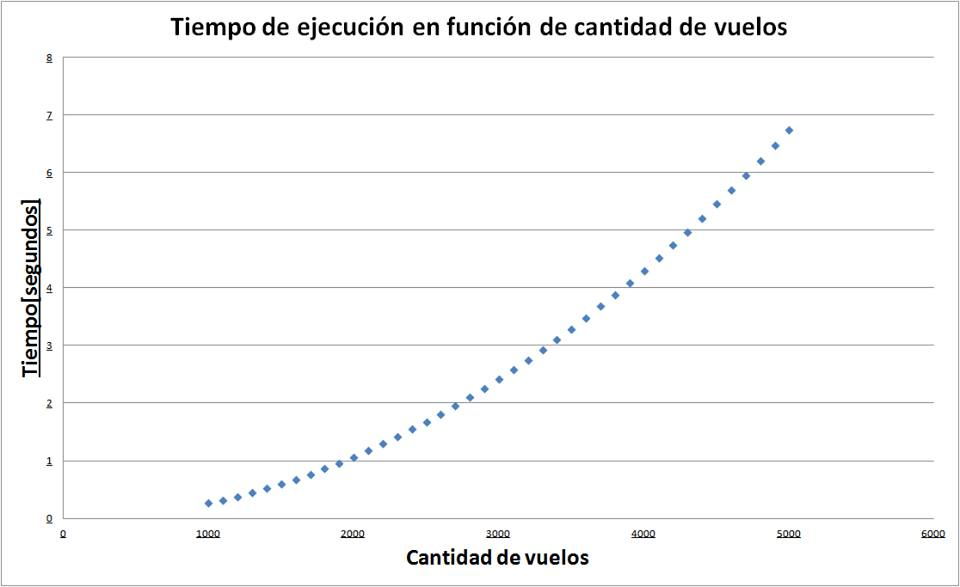
\includegraphics[scale=0.5]{imagenes/graph2-1.jpg}
\caption{Gráfico de tiempo de ejecución para instancias de tamaño creciente}
\end{figure}

A simple vista podemos ver que la curva descripta en el gráfico no es lineal (crece \textit{más rápido}) y podemos sospechar, dada la demostración presentada previamente, que se trata de una función cuadrática. Para intentar proveerle mayor grado de certeza a nuestra sospecha, presentamos el siguiente gráfico:

\begin{figure}[H]
\centering
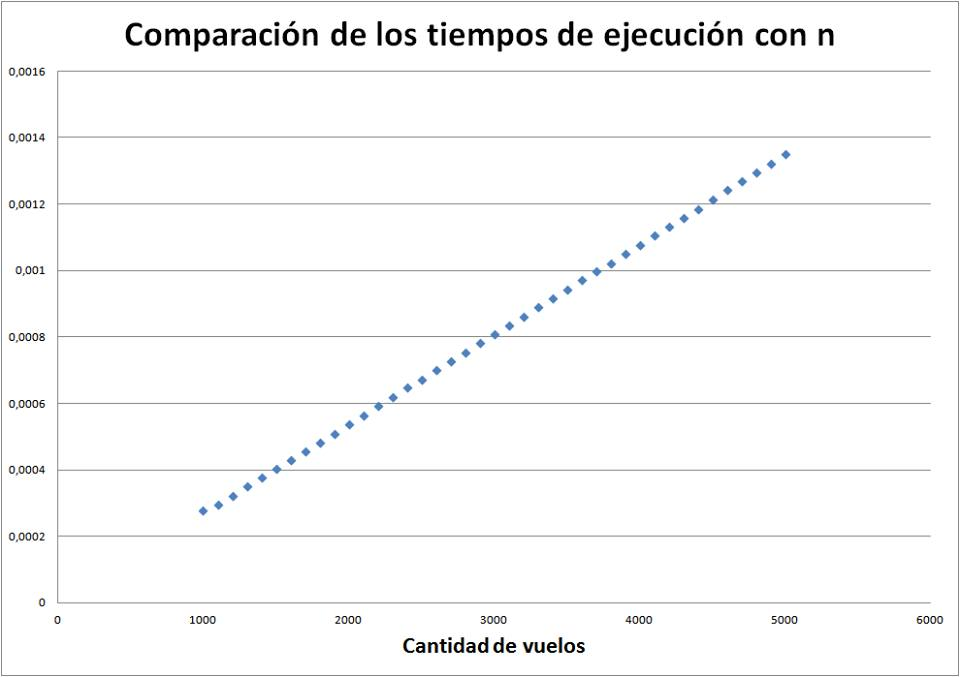
\includegraphics[scale=0.5]{imagenes/graphn.jpg}
\caption{Gráfico de comparación de tiempo de ejecución con $n$}
\end{figure}

Para la confección de este último gráfico tomamos los tiempos de ejecución y los dividimos por la cantidad de vuelos. Esta operación produjo una función aparentemente lineal lo cual nos brinda mayor certeza sobre la complejidad propuesta (al menos para instancias de tamaño entre 1000 y 5000).

\subsection{Adicionales}
Si cada vuelo perteneciera a una aerolínea distinta, esto no afectaría la complejidad
de nuestro algoritmo: lo que deberíamos hacer para lidiar con este nuevo problema 
sería tener un arreglo, $aerolinea$ que para cada vuelo (los vuelos están numerados de 1 a $n$) nos
diga (en $O(1)$) a qué aerolínea corresponde. Entonces, cuando armamos la matriz de 
adyacencias para representar a nuestro grafo dirigido, vamos a tener que considerar esta
nueva restricción para que efectivamente sea posible combinar cada par de vuelos. Bajo las
nuevas condiciones impuestas, para decir que hay forma de combinar dos vuelos $a$ y $b$, 
cuando armemos la matriz de adyacencia, vamos a tener que considerar dos posibilidades: 
\begin{enumerate}
	\item si $aerolinea[a] = aerolinea[b]$, que el destino del vuelo $a$ sea el mismo que 
	el origen de vuelo $b$ y que haya por lo menos \textbf{una} hora de diferencia entre la llegada 
	a su destino del vuelo $a$ y la salida de su origen del vuelo $b$ (aquí relajamos una 
	condición, pues antes había que chequear que hubieran al menos dos horas de diferencia).
	\item si $aerolinea[a] \neq aerolinea[b]$, que el destino del vuelo $a$ sea el mismo que
	el origen del vuelo $b$, que haya por lo menos 2 horas de diferencia entre la llegada a su
	destino del vuelo $a$ y la salida del vuelo $b$ (igual que antes).
\end{enumerate}


%% ================
%% ================ problema 2 =========================0
%% ================

\section{Problema 2- Caballos salvajes}

\subsection{Descripción del problema}

El problema planteado consiste en, dado un tablero de ajedrez cuadrado con n casillas de lado con algunas casillas ocupadas por caballos, devolver (si es posible)una casilla a la cual puedan llegar todos los caballos minimizando la cantidad total de saltos que hacer para llegar a ella. Notar que los caballos sólo podrán realizar sus movimientos permitidos por el reglamento de ajedrez\footnote{\url{http://es.wikipedia.org/wiki/Caballo_(ajedrez)}}.

Veamos algunas instancias para esclarecer este punto:

\begin{figure}[H]
\centering
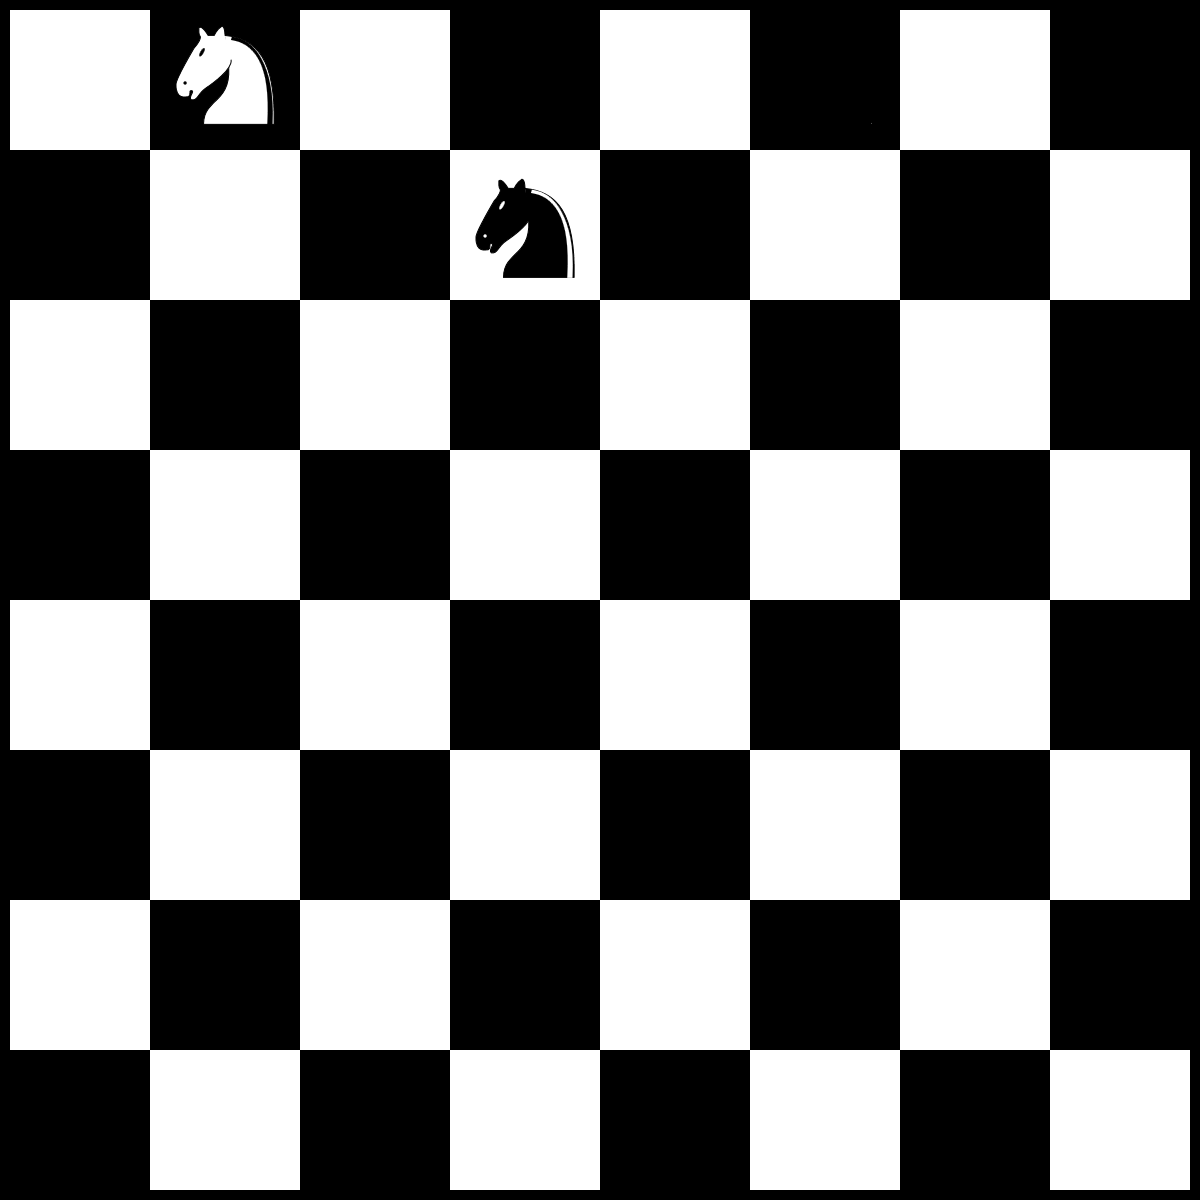
\includegraphics[scale=0.25]{imagenes/chess1.jpg}
\caption{}
\end{figure} 

Para representar esta instancia nuestro algoritmo recibirá una entrada así:

8 2 \\
1 2\\
2 4\\

En donde la primera linea tendrá la cantidad de filas (y columnas) del tablero ($n$) seguido de un entero $k$ con la cantidad de caballos presentes (2 en este caso). Seguida a esta linea, habrá $k$ lineas con la fila y la columna (numeradas de 1 a n, siendo el (1,1) la esquina superior izquierda)
En este primer caso es bastante claro que en 1 solo salto total pueden encontrarse ambos caballos. Sin embargo hay 2 posibles soluciones. Devolvemos cualquiera de ellas, en nuestro caso será

1 2 1

Esto se interpreta como "Se encuentran en la casilla (1,2) en 1 salto".

Veamos ahora otra instancia con un tablero más pequeño:

\begin{figure}[H]
\centering

\includegraphics[scale=0.35]{imagenes/chess-nosol.jpg}
\caption{}
\end{figure} 

En este caso la entrada será

3 2\\
1 2\\
2 2\\

y el problema no podrá ser resuelto devoliendo entonces \textbf{no}. Esto sale simplemente de notar que desde ninguna posición distinta de la (2,2) puede llegarse a la (2,2) y a su vez, desde la (2,2) no hay ninguna posición válida a la cual moverse.

En las secciones posteriores presentaremos y explicaremos un procedimiento que permita devolver un resultado para cada instancia de este tipo, demostraremos su correctitud y veremos además que puede hacerlo en la complejidad temporal solicitada $O(k.n^2)$

\subsection{Ideas para la resolución}

Para resolver este problema pensamos al tablero de ajedrez como un grafo. Cada casilla será un nodo y sólo habrá arista entre dos nodos u y v si es posible llegar de u a v en un solo salto de caballo.

Como las aristas no tienen peso (todas significan un salto), es posible, mediante BFS\footnote{"Introduction to algorithms" 3rd Ed. Thomas H. Cormen, Charles E. Leiserson, Ronald L. Rivest, and Clifford Stein- Section 22.2} encontrar, desde una casilla, el camino mínimo en saltos hacia el resto.  

Si repetimos este procedimiento para cada casilla con caballos, sabremos, para cada caballo, en cuántos saltos puede llegar a una casilla del tablero (si es que puede). 

Luego, si en cada nodo, además de su posición, almacenamos quién lo visitió y acumulamos los saltos requeridos para llegar a él(distancia a la casilla origen en BFS) , al final tendremos en cada uno del los $n^2$ nodos la información necesaria. Basta encontrar aquel que fue visitado por todos que tenga cantidad de saltos necesarios mínima. Si no existe, entonces no habrá solución. Si existe, devolvemos su posición y la cantidad de saltos totales.

En resumen, el procedimiento propuesto consiste en aplicar k veces BFS ($O(n^2)$) al tablero y luego buscar en una matriz de $n^2$ el valor buscado ($O(n^2)$). Basta probar que este procedimiento es correcto y que la complejidad de nuestra implementación se ajusta a las cotas planteadas.

\subsection{Demostración de correctitud}
Analicemos nuestro código implementado por partes. Veamos primero el BFS:

A continuación, introducimos un fragmento de código para mostrar correctitud de nuestro algoritmo

\begin{verbatim}
void BFS(vector<vector<casilla> >& graph, int i, int j, int n) 
{

    queue<pair<int,int> > queue; //creo cola bfs

    //visito nodo origen, incremento su kVisitado y lo pusheo
    graph[i][j].visited = true;
    graph[i][j].kVisitado ++;
    queue.push(make_pair(i,j));


	pair<int,int> src;

    while(!queue.empty())
    {
      
        src = queue.front();
        queue.pop();

       
		visitarAdj(graph, queue, src.first,src.second,n);

    }
}

\end{verbatim}


Este código es prácticamente \textit{verbatim} del pseudocódigo de BFS. Toma un tablero (grafo) y una posición (i,j) inicial. De hecho la única diferencia está en la función \textit{visitarAdj}. 

La copia de la función se encuentra en el apéndice final.Esta recibe una posición (i,j) del tablero y la distancia al padre (i.e. a cuántos saltos está esa posición del origen), para todas las posiciones de salto válidas (i.e. cuyas coordenadas quedan dentro del tablero y correspondan a una movida de caballo), si aún no fue visitada, llama a función VisitarNodo de esa posición. Esta función toma un nodo y actualiza sus campos así:

\begin{verbatim}
void visitarNodo(casilla& nod, int distanciaPadre){ //actualiza los campos de un nodo dado al visitarlo por BFS
	            nod.visited = true;
                nod.kVisitado++;
                nod.distSrc= distanciaPadre+1;
                nod.saltosNecesarios+=nod.distSrc;
	}
\end{verbatim}

Esta función entonces visita al nodo, le aumenta el campo kVisitado (será utilizado posteriormente para saber cuántos caballos visitaron ese nodo), actualiza su distancia a la casilla de partida y suma esta distancia a la cantidad de saltos totales requeridos para llegar a este nodo. 

Vemos entonces que la modificación que realizamos sobre el BFS original no es más que agregar campos en los nodos y, en lugar de usar una matriz para chequear adjacencia, directamente calculamos las posiciones adjacentes en cada paso. Por este motivo podemos utilizar la postcondición de BFS.

Entonces podemos decir que nuestro BFS hace exactamente lo que queremos. Visita cada nodo una vez y nos garantiza que desde el origen hacia ese nodo la distancia es mínima. 

Con esto en mente, dado que en cada casilla acumulamos la cantidad de saltos requeridos para llegar a ella, aquella que sume la menor cantidad y sea visitada por los k caballos será una solución óptima posible. Cualquier otra solución óptima es igual de buena y no puede haber otra mejor porque justamente BFS garantiza que cada vez que vista a un nodo lo hace en la menor cantidad de saltos posibles.

Para poder ejecutar este BFS tendremos que inicializar el grafo de forma adecuada. Para ello empleamos una matriz en donde cada posición representa una posición del tablero y contiene los campos mencionados(visited, kVisitado, distSrc (distancia a la casilla origen) y saltosNecesarios (acumula los saltos necesarios para llegar de todos los que lo visitaron) ).
Para poder repetir este proceso es necesario limpiar algunos campos de los nodos. Estos son el campo que chequea si fue visitado (visited) y la distancia al origen. El resto de los campos queremos que conserven sus resultados (kVisitado y saltosNecesarios) para obtener de ellos la solución.  

Una vez hecho esto para las k posiciones de los caballos tendremos en los nodos lo que queremos. Buscamos en el tablero aquella posición cuyo campo kVisitado sea igual a la cantidad de caballos en el tablero y su saltosNecesarios sea mínimo y, entonces, esta posición será una de las posibles óptimas.

\subsection{Demostración de complejidad}

Recordemos qué hace nuestro código:

\begin{enumerate}

\item Leer la entrada
\item Construir tablero (matriz). $(O(n^2))$
\item Realizar K veces BFS sobre el tablero $(O(k(n^2)))$. Si bien en este caso la cantidad de aristas es constante, en el peor caso BFS tiene que mirar todas las posibles aristas, que en un peor caso son $n^2$.  Antes de cada nueva ejecución es necesario limpiar el tablero $(O(n^2))$.
\item Buscar la solución en el tablero ($(O(n^2))$)

\end{enumerate}

Se puede ver que la complejidad es $n^2+2(k(n^2))+n^2 = (O(k(n^2)))$. 

Para las operaciones de pares y vectores se usan pair\footnote{\url{http://en.cppreference.com/w/cpp/utility/pair}} y vector\footnote{\url{http://en.cppreference.com/w/cpp/container/vector}} de la std con sus operaciones de acceso a un elemento en tiempo constante y, en el caso de vector, de resize en tiempo lineal respecto del parámetro. También empleamos queue \footnote{\url{http://en.cppreference.com/w/cpp/container/queue}} con sus operaciones push y pop en tiempo constante.

\subsection{Tests de complejidad}
En esta sección analizamos empíricamente la complejidad temporal de nuestro algoritmo.

Dada la forma en la que nuestro algoritmo procesa las instancias, no hemos podido encontrar alguna distribución particular de los caballos en un tablero que nos permita procesar esa entrada más rápido que cualquier otra entrada de igual tamaño e igual cantidad de caballos. Al procesar nuestro algoritmo a partir de una casilla el BFS completo para la misma, cualquier entrada con K caballos hará K BFS. Vale notar el caso extremo en el los K caballos estén en la misma casilla inicial. En este caso repetirá la ejecución del BFS K veces. 
Evidentemente esta es una optimización posible (analizar los casos de posiciones repetidas y evitar repetir el mismo bfs puesto que ya conocemos qué casillas visitará y cuántos saltos aportará) que no hemos llevado a cabo. 

Dicho esto, presentaremos entonces 3 gráficos para instancias de diferente tamaño en donde los caballos fueron colocados al azar en un tablero. Veremos que la complejidad cumple con la cota establecida, comportándose de forma lineal respecto de K y también respecto de K.n. 

\begin{figure}[H]
\centering
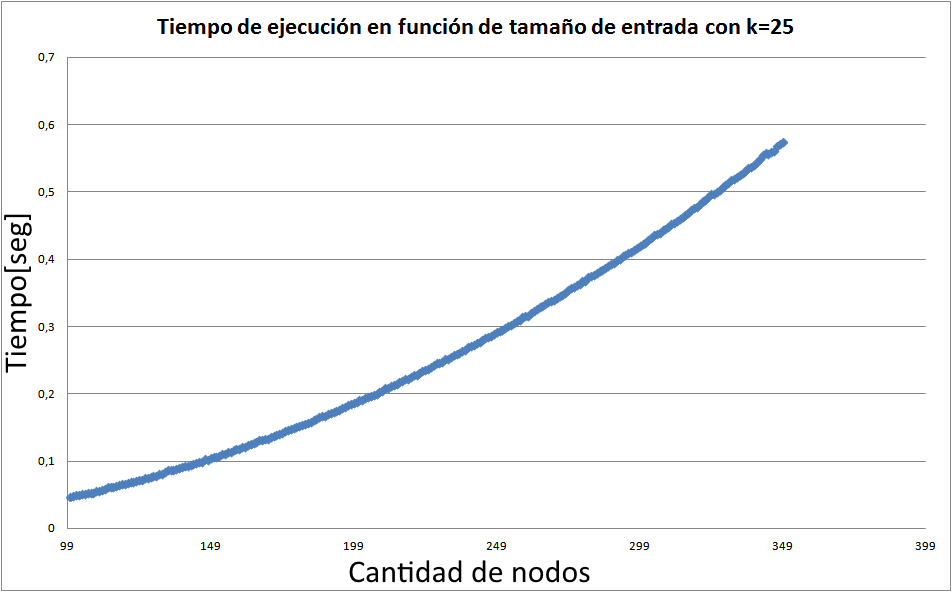
\includegraphics[scale=0.4]{imagenes/orig.jpg}
\caption{Gráfico de tiempos de ejecución para entradas de tamaño creciente con k fijo}
\end{figure} 

En este gráfico apreciamos cómo, para un k fijo, el tiempo de ejecución crece \textit{más rápido} que una función lineal al incrementar la cantidad de filas (y columnas) en el tablero. Dado que propusimos una complejidad de orden $kn^2$, si dividimos los tiempos obtenidos por $kn$ para cada $n$ deberíamos apreciar una función lineal, que es, efecivamente lo que se observa en el siguente gráfico:


\begin{figure}[H]
\centering
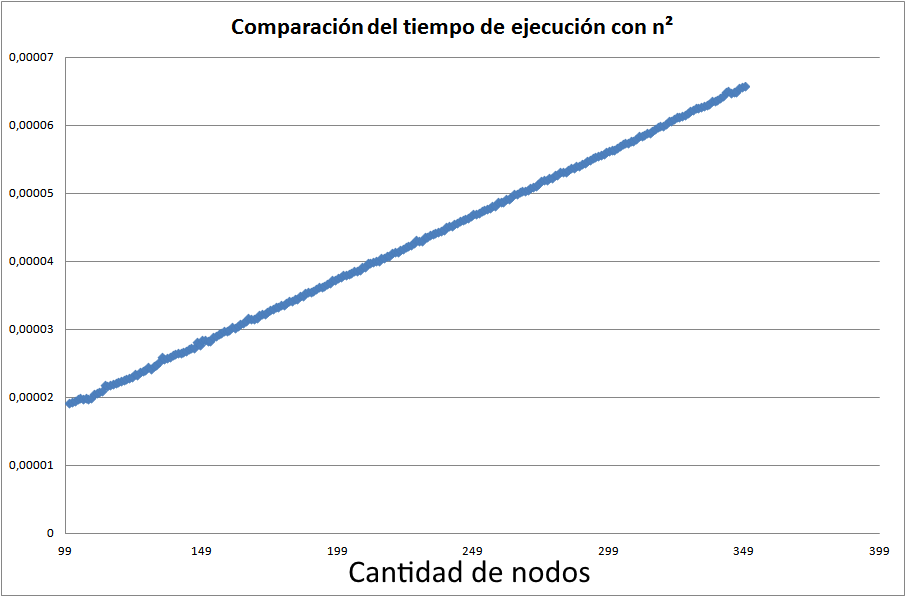
\includegraphics[scale=0.4]{imagenes/n2.jpg}
\caption{Comparación de tiempo de ejecución con $k.n$}
\end{figure} 

Ya vimos que el tiempo de ejecución evoluciona de forma cuadrática para $n$ fijando un k. Ahora queremos ver, para terminar de probar nuestra cota de complejidad, que el tiempo crece de forma lineal con k. Para ello, fijamos un las filas y columnas del tablero e incrementamos la cantidad de caballos en él. Obtuvimos el siguiente gráfico:

\begin{figure}[H]
\centering
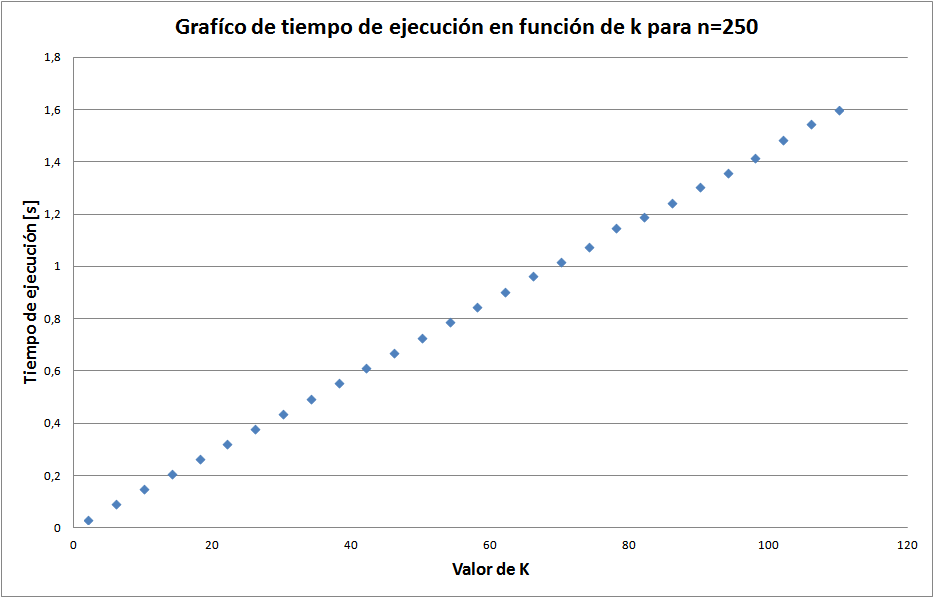
\includegraphics[scale=0.4]{imagenes/k.jpg}
\caption{Gráfico de tiempo de ejecución en función de $k$ con n fijo}
\end{figure} 

Basándonos exclusivamente en la observación del gráfico, podemos notar la relación lineal entre k y el tiempo de ejecución para un n fijo.

\subsection{Adicionales}

Para una modificación del algoritmo nos requirieron una solución para el mismo problema en el caso de que sean alfiles en lugar de caballos las piezas en el tablero.

En esta nueva situación los nodos adyacentes a una casilla ya no son constantes como en el caso de los caballos sino que dependen del tamaño del tablero (puesto que el alfil se mueve en forma diagonal por el mismo). De esta manera, la función que visista los nodos adyacentes ya no podrá mirar una cantidad constante de vecinos sino que dependerá de la casilla que la llame. Asi, en el peor caso (alguna casilla central), tendrá que visitar 2n-2 vecinos. Si bien la complejidad teórica no se modifica (BFS sigue tardando $n^2$), la función que visita a los adyacentes tendrá que iterar sobre las 2 diagonales respecto de la posición en la que se encuentre el alfil para visitar a sus vecinos.


\subsection{Apéndice: Código relevante}

A continuación presentamos las funciones relevantes que implementamos para el problema: 

\begin{verbatim}
bool esValida(int x, int y, int n){ //chequea si una posición del tablero es válida
    return ( x >= 0 && x < n && y >= 0 && y < n);
}

void visitarAdj(vector<vector<casilla> >& graph, queue<pair<int,int> >& queue, int i, int j, int n){ //visita los adyacentes a la casilla [i,j] en el graph y los pushea en queue

           pair<int,int> temp;

            if( esValida(i+2,j+1,n) && !(graph[i+2][j+1].visited) ){
				visitarNodo(graph[i+2][j+1], graph[i][j].distSrc);
				temp=make_pair(i+2,j+1);
				queue.push(temp);
            }
            if( esValida(i+2,j-1,n) && !(graph[i+2][j-1].visited) ){
				visitarNodo(graph[i+2][j-1], graph[i][j].distSrc);
				temp=make_pair(i+2,j-1);
				queue.push(temp);
            }
            if( esValida(i-2,j+1,n) && !(graph[i-2][j+1].visited) ){
				visitarNodo(graph[i-2][j+1], graph[i][j].distSrc);
				temp=make_pair(i-2,j+1);
				queue.push(temp);
            }
            if( esValida(i-2,j-1,n) && !(graph[i-2][j-1].visited) ){
				visitarNodo(graph[i-2][j-1], graph[i][j].distSrc);
				temp=make_pair(i-2,j-1);
				queue.push(temp);
            }
            if( esValida(i+1,j+2,n) && !(graph[i+1][j+2].visited) ){
				visitarNodo(graph[i+1][j+2], graph[i][j].distSrc);
				temp=make_pair(i+1,j+2);
				queue.push(temp);
            }
            if( esValida(i-1,j+2,n) && !(graph[i-1][j+2].visited) ){
				visitarNodo(graph[i-1][j+2], graph[i][j].distSrc);
				temp=make_pair(i-1,j+2);
				queue.push(temp);
            }
            if( esValida(i+1,j-2,n) && !(graph[i+1][j-2].visited) ){
				visitarNodo(graph[i+1][j-2], graph[i][j].distSrc);
				temp=make_pair(i+1,j-2);
				queue.push(temp);
            }
            if( esValida(i-1,j-2,n) && !(graph[i-1][j-2].visited) ){
				visitarNodo(graph[i-1][j-2], graph[i][j].distSrc);
				temp=make_pair(i-1,j-2);
				queue.push(temp);
            }
        }

int main() {


	///leer entrada
	int n,k,f,c;
	cin>>n;
	cin>>k;
	pair<int,int> cab;
	vector<pair<int,int> >kCab(k);
	for(int i=0;i<k;++i){
		cin>>f;
		cin>>c;
        kCab[i]=make_pair(f-1,c-1);
		//cout<<cab.first<<" "<<cab.second<<endl;
		//kCab.push_back(cab);
       // cout<<"Pares: "<<kCab[i].first<<" "<<kCab[i].second<<endl;
		}

	///inicializo nodos
	vector<vector<casilla> > graph(n);
	for(int i=0;i<n;i++){
		graph[i].resize(n);
		for (int j=0;j<n;j++){
                graph[i][j].visited=false;
                graph[i][j].kVisitado=0;
                graph[i][j].saltosNecesarios=0;
                graph[i][j].distSrc=0;
		}
    }

	for(int z=0 ; z<k ; ++z){ ///K veces BFS

		BFS(graph, (kCab[z]).first, (kCab[z]).second,n);

		// limpio campos del bfs para la próxima corrida (n^2)
		for(int i = 0; i < n; ++i){
			for(int j=0;j<n;++j){
				(graph[i][j]).visited = false;
				(graph[i][j]).distSrc = 0;
			}
		}

    }

	ImprimirSolucion(graph, k);

    return 0;
}


\end{verbatim}

%% ================
%% ================ problema 3 =========================0
%% ================
\clearpage
\section{Problema 3 - La comunidad del anillo}

\subsection{Descripción del problema a resolver}
La empresa \texttt{AlgoNET} nos contrató para que le brindemos una 
solución algorítmica a un problema de redes. Nuestro cliente quiere ofrecer
un sevicio particular sobre una red existente de computadoras. La red cuenta
con un conjunto de conexiones entre pares de computadoras, donde cada 
conexión tiene un costo asociado. El objetivo es elegir un subconjunto de 
conexiones y de equipos (que funcionarán como servidores) tales que:
\begin{enumerate}
  \item El conjunto de servidores deberá conformar un anillo
  \item Todo equipo debe quedar conectado al anillo de servidores vía un 
        enlace directo o pasando a través de otros equipos en el medio
  \item La suma total de los costos de todos los enlaces utilizados debe
        ser lo mínima posible
  \item El algoritmo debe tener una complejidad estrictamente mejor que $O(n^3)$
  \item El algoritmo debe detectar los casos en los que no haya solución
\end{enumerate}

El formato de entrada contiene una instancia del problema. La primera línea 
contiene un entero positivo $n$ que indica la cantidad de equipos de la red
(numerados de 1 a $n$), y un entero no negativo $m$ que corresponde a la 
cantidad de enlaces disponibles. A esta línea le siguen $m$ líneas, una para
cada enlace, con el formato \texttt{e1 e2 c} donde \texttt{e1} y \texttt{e2}
representan los equipos en los extremos del enlace en cuestión (ambos enteros
entre 1 y $n$) y \texttt{c} es el costo por utilizar dicho enlace. En caso de
haber solución, la salida tiene el formato \texttt{C Ea Er} donde \texttt{C} es
el csoto de la solución dada y \texttt{Ea} y \texttt{Er} son los enlaces 
utilizados por el anillo y para el resto de la red, respectivamente. A esta línea
le siguen \texttt{Ea} líneas, una para cada enlace utilizado en el anillo y luego
\texttt{Er} líneas, una para cada enlace utilizado fuera del anillo, todas con el 
formato \texttt{e1 e2} donde \texttt{e1} y \texttt{e2} representan los extremos
del enlace en cuestión. Si hay más de una solución óptima, se puede devolver 
cualquier, y si no hay solución se debe devolver la palabra \texttt{no}. A 
continuación, mostramos un ejemplo de una posible instancia.

\begin{minipage}[t]{0.4\textwidth}
\begin{Verbatim}[frame=single,framesep=1cm,label= Ejemplo de entrada: instancia 1]
8 10
1 2 1
2 6 1
2 3 5
2 7 2
6 7 1
7 5 3
3 5 8
5 4 2
5 8 2
4 8 10
\end{Verbatim}
\end{minipage}
\hfill
\begin{minipage}[t]{0.4\textwidth}
\begin{Verbatim}[frame=single,framesep=1cm,label= Ejemplo de salida: instancia 1]
17 3 5
2 6 1
6 7 1
2 7 2
1 2 1
5 4 2
5 8 2
7 5 3
2 3 5
\end{Verbatim}
\end{minipage}

A continuación, presentamos una representación del problema, visto como 
un grafo: cada nodo es un equipo y cada arista es una conexión entre 
algún par de computadoras, y tiene un costo asociado a dicha conexión, 
seguido de tres posibles formas de elegir los subconjuntos de equipos y 
conexiones requeridos por el problema

\begin{figure}[H]
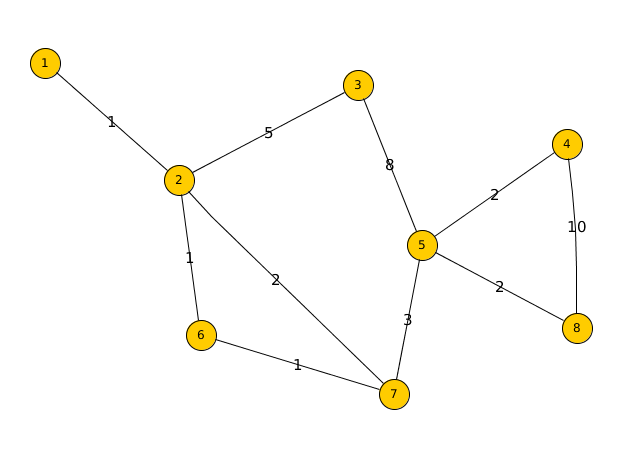
\includegraphics[scale=1]{imagenes/equipos2.png}
\caption{Red de equipos}
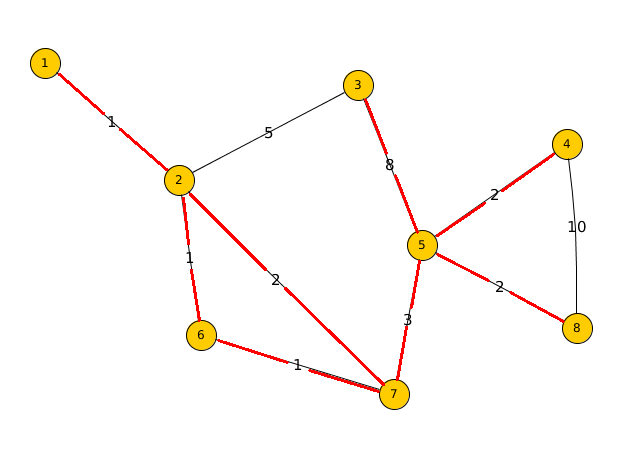
\includegraphics[scale=1]{imagenes/equipos3.png}
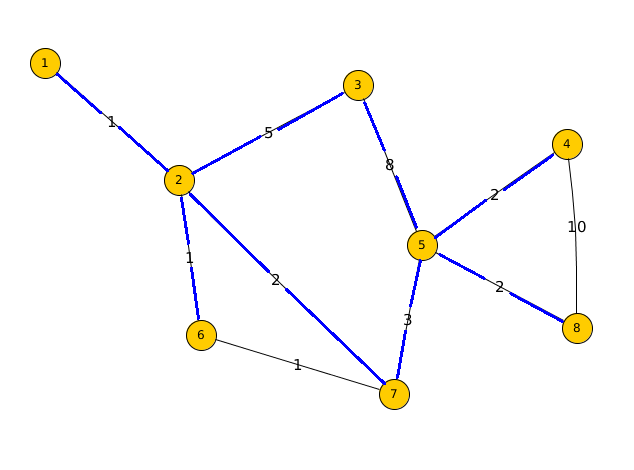
\includegraphics[scale=1]{imagenes/equipos4.png}
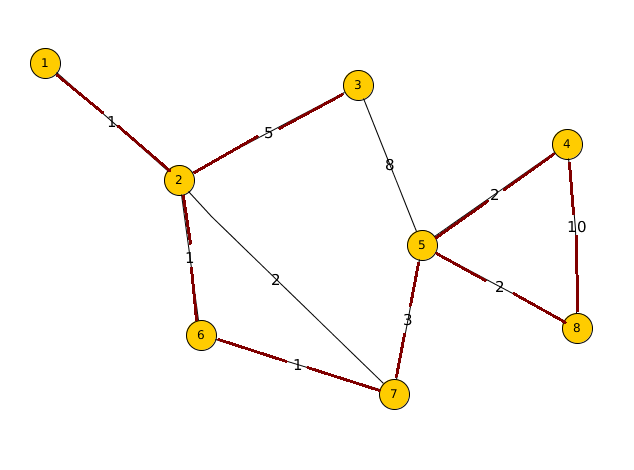
\includegraphics[scale=1]{imagenes/equipos5.png}
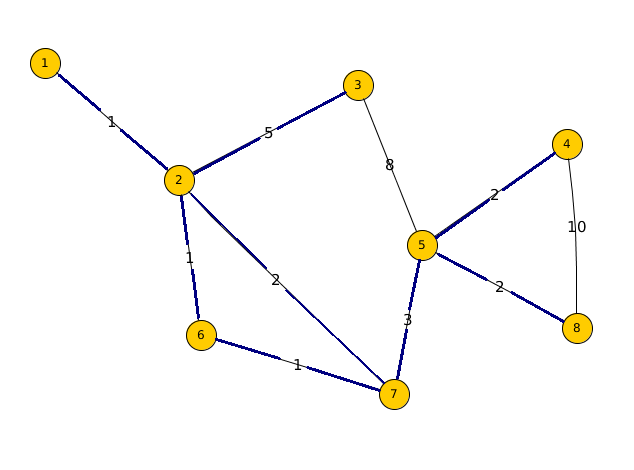
\includegraphics[scale=1]{imagenes/equipos7.png}
\caption{Soluciones de costo C = 20 (rojo), C = 24 (azul), C = 25 (marrón)
         C = 17 (azul oscuro) respectivamente}
\end{figure}

Se puede observar que las tres soluciones presentadas en la figura 1.1.2 
son efectivamente soluciones porque todas presentan algún circuito de
servidores, y en todos los casos, todas las computadoras de la red están 
conectadas con los servidores con conexiones directas o a través de conexiones
con otros equipos. Sin embargo, no todas estas soluciones son óptimas: una 
tiene costo 20, otra 24 otra 25 y otra 17. Es decir, que para este caso en particular,
nuestro algoritmo debería devolver como solución los servidores 2, 6, 7 y
los enlaces que están marcados en azul oscuro en la figura 1.1.2.

\subsection{Ideas desarrolladas para la resolución}
A partir del ejemplo presentado en la sección anterior y de algunos otros,
observamos que en todos los casos, todos los enlaces que conformaban el 
árbol generador mínimo (AGM) del grafo generado por nuestra red de equipos
estaban incluidos en la solución óptima del problema. En nuestro ejemplo,
el AGM sería:

\begin{figure}[H]
\centering
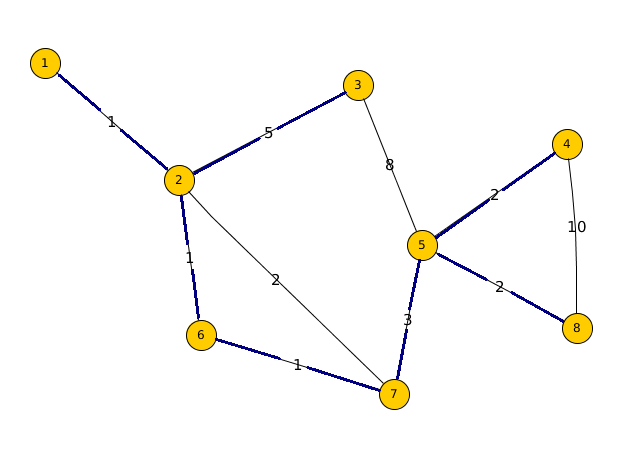
\includegraphics[scale=1]{imagenes/equipos6.png}
\caption{Árbol Generador Mínimo del grafo del ejemplo de la figura 1.1.1}
\end{figure} 

Entonces, pensamos que posiblemente esto siempre sucediera, al menos siempre
que existiera alguna solución. Así es que,
intentamos probar que tomando el AGM del grafo en cuestión y luego 
agregándole la arista de menor peso de las que no estuvieran incluidas
en el AGM, el grafo generado sería una solución (sería un grafo con algún 
ciclo y todos los nodos estarían conectados con algún nodo del conjunto de 
nodos que conformaban el ciclo en el grafo) y que sería óptima (la suma
total de los pesos de los enlaces sería lo mínima posible). La demostración
de que esto es así esta en la sección en la que demostramos correctitud. \\
Entonces, a continuación describimos los pasos que nuestro algoritmo
efectuará para resolver el problema planteado:

\begin{enumerate}
  \item generar un grafo $G$ en donde cada nodo sea un equipo y cada arista un
        enlace entre un par de equipos, con un costo asociado igual al costo
        que hay que pagar por el ancho de banda empleado por dicha conexión
  \item chequear si el grafo $G$ es conexo. Si no lo es, entonces el problema
        no tendrá solución
  \item si el grafo $G$ es conexo, generar el árbol generador mínimo $T$ del grafo
        $G$ y chequear que este AGM no consuma todas las aristas del grafo $G$ (de
        lo contrario, no quedaría ninguna arista libre para agregar a $T$ y formar
        el ciclo que queremos y no habría solución).
  \item buscar el menor de los enlaces que aparece en el grafo $G$ pero que no 
        aparece en el árbol generador mínimo $T$. Llamemos a ese eje $e$.
  \item agregamos el eje $e$ al AGM $T$. Queda así formado el grafo $G' = T + e$,
        que es un grafo conexo y tiene un único ciclo. Además, cumple con todo lo
        que nos pide el enunciado del problema
  \item devolvemos la suma total de los costos de todas las conexiones que son
        utilizadas por nuestro grafo $G'$ y, por otro lado, devolvemos los enlaces
        que conforman nuestro anillo de servidores y el resto de los enlaces 
        de nuestra solución
        
\end{enumerate}

\subsection{Demostración de Correctitud}
Para demostrar la correctitud de nuestro algoritmo, tenemos que demostrar que los
pasos descriptos en la sección anterior para la resolución del problema 
efectivamente nos conducen a la generación de una solución correcta. Entonces,
repasando las ideas ya expuestas, lo que planteamos es que se puede llegar a una
solución óptima a partir de generar el AGM $T$ de nuestro grafo $G$ y luego generar
el grafo $G' = T + \{e\}$, donde $e$ es el eje de menor costo que esta en $G$ y
no en $T$. Pero lo que nos pide el enunciado es que generemos, a partir del grafo $G$,
otro grafo $G''$ tal que $G''$ sea conexo, que la suma
total de los costos de sus ejes sea lo mínima posible y que contenga un único ciclo 
(ya que si tuviera 
más de un ciclo, como todos los ejes son de peso positivo, podríamos quitar los ejes 
necesarios para que sólo quede un único ciclo y lograríamos así cumplir los requisitos
del problema, pero consiguiendo un costo total menor). Entonces, demostrando la 
siguiente proposición, estaríamos demostrando nuestro método empleado para la resolución
es efectivamente correcto:

\newtheorem{prop}{Proposición}
\begin{prop}
Dado un grafo G conexo, con T un AGM de G y S el conjunto de todos los árboles
generadores de G y $e$ el mínimo eje perteneciente a $G \backslash T$ vale que: 
$costo(T+e) = \min\limits_{\substack{T' \in S \\ f \in G \backslash T'}} costo(T'+f)$
\end{prop}
\begin{proof}[Demostración de la Proposición 1] 
Primero, vamos a demostrar dos lemas: 
\begin{enumerate}
  \item si $S_{opt}$ es una solución óptima al problema (es algún subgrafo conexo  de G
		con algún ciclo), entonces $S_{opt}$ contiene a algún AGM de G.
		
		\begin{proof}[Demo de 1]
		Sea $S_{opt}$ una solución óptima para el probelma. Entonces, $S_{opt}$ tiene un único ciclo
		porque si tuviera más de uno, como todos los ejes son de peso positivo, podríamos quitar
		los ejes necesarios para que quede un único ciclo, y quedaría una solución $S'_{opt}$ mejor que $S_{opt}$.
		Consideremos una solución óptima: $S_{opt} = T + \{k\}$ donde $T$ es algún árbol que visita 
		todos los nodos de $G$. Y por otro lado consideremos un AGM de $G$: $T'$. Seguro que en el ciclo
		que se forma en $S_{opt}$ hay algún eje $e$ tal que $e \not\in T'$ puesto que $T'$ es un árbol y 
		por lo tanto no puede tener ciclos. Entonces, consideremos esta otra solución no necesariamente 
		óptima para nuestro problema: $S' = T' + \{e\}$. Entonces, por un lado, como $S_{opt}$ es una solución
		óptima y $S'$ no necesariamente, vale que peso($S_{opt}$) $\leq$ peso($S'$). Por otro lado, como $e$
		esta incluido en el ciclo que se forma en $S_{opt}$, podemos reescribir a $S_{opt}$ como 
		$S_{opt} = T'' + \{e\}$ donde $T''$ es un árbol no necesariamente mínimo, que visita todos los nodos
		de $G$. Luego, vale que peso($T'$) $\leq$ peso($T''$), pues $T'$ es un AGM de $G$. Entonces, también
		podemos concluir que peso($S'$) $=$ peso($T' + \{e\}$) $\leq$ peso($T''+\{e\}$) $=$ peso($S_{opt}$).
		Entonces, peso($T'' + \{e\}$) $=$ peso($S_{opt}$) = peso($S'$) $=$ peso($ T' + \{e\}$) donde $T'$ es un
		AGM de $G$ y $T''$ un AG de $G$. Pero como peso($e$) $=$ peso($e$), tiene que valer también que
		peso($T'$) $=$ peso($T''$). Pero entonces, como $S_{opt} = T'' + \{e\}$, $T''$ tiene que ser un AGM de
		$G$. Por lo tanto, $S_{opt}$ seguro que contiene un AGM de $G$.
		\end{proof}
  
  \item dado un grafo G, si tomo algún AGM de G entonces la longitud de la mínima 
        arista de las que están en G $\backslash$ T es siempre la misma.
        
        \begin{proof}[Demo de 2]
		Supongamos que $T$ y $T'$ son dos AGM's distintos y que la arista de menor longitud 
		que queda en $G \backslash T$ es $e$ mientras que la de menor longitud que queda en
		$G \backslash T'$ es $f$ y además supongamos que peso($e$) $<$ peso ($f$). Entonces,
		como $T$ y $T'$ son árboles y están construidos sobre el mismo grafo $G$, sabemos que
		tienen la misma cantidad de aristas y $e \in T'$ pues de lo contrario $e$ sería el mínimo
		eje perteneciente a $G \backslash T'$ y no $f$.\\
		Ahora, supongamos que formamos el grafo 
		$H = T + \{e\}$. Se forma un ciclo: $e, e_{1}, e_{2} \dots e$, donde long($e$) $\geq$ 
		long($e_{i}$) (puesto que de lo contrario, podríamos obtener el árbol $T + \{e\} - \{e_{i}\}$, de 
		longitud menor que T) y además, \textbf{no todos} 
		los ejes $e_{i}$ están incluidos en $T'$, puesto que por hipótesis, $e \in T'$ y entonces
		$e$ formaría un ciclo en $T'$ con $e_{1} e_{2} \dots$, lo cual es absurdo porque $T'$ es un
		árbol y no puede tener ciclos.
		Luego, si $e_{k} \not\in T'$, como long($e_{k}$) $\leq$ long($e$) $<$ long($f$), $f$ no 
		era la arista más chica de $G \backslash T'$ (Absurdo). Entonces, concluimos que 
		peso($e$) $\geq$ peso($f$). Haciendo la misma demostración, pero con la hipótesis de que
		peso($f$) $<$ peso($e$) obtendríamos exactamente la desigualdad opuesta. 
		Entonces, concluimos que peso($e$) $=$ peso($f$) siempre, lo cual implica que 
		la longitud de la mínima arista de las que están en $G \backslash T$ tiene siempre de
		la misma longitud, sin importar que AGM $T$ se elija.
		\end{proof}
\end{enumerate}
Entonces, si consideramos cualquier AGM $T$ de $G$, por lo demostrado en el punto 2, la
longitud de la mínima arista de las que quedan (llamémosla $e$) es siempre la misma.
Entonces, para cualquier AGM $T$ que elijamos, la longitud del grafo $ G'' = T + \{e\} $
también es siempre la misma, porque todos los AGM's de un grafo tienen que tener la misma
longitud. Entonces, sea $G_{opt}$ la solución óptima del problema para el grafo $G$. 
Por lo visto en el punto 1, $G_{opt}$ contiene un AGM de $G$. Supongamos que contiene 
al AGM $T$. Entonces, como además sabemos que $G_{opt}$ tiene un único ciclo (porque todas las 
aristas del grafo $G$ tienen peso positivo, si $G_{opt}$ tuviera dos o más ciclos distintos,
podríamos quitar un eje distinto de todos estos ciclos menos uno, y tendríamos una solución del problema 
mejor que la óptima, pues habríamos quitado aristas de peso positivo y el grafo seguiría siendo conexo
y con algún ciclo), seguro que
$G_{opt} = T + \{e\}$ para algún eje $e$ que está en $G$ pero no en $T$. Pero para que 
$G_{opt}$ sea de longitud mínima, la longitud de $e$ debe ser menor o igual que la 
longitud de $f$ para cualquier eje $f \in G \backslash T$. Entonces, 
$G_{opt} = T + \{e\}$ donde $T$ es algún AGM de $G$ y $e$ es un eje perteneciente a
$G \backslash T$ y de longitud mínima en ese conjunto, y además la longitud de
$G_{opt} = T + \{e\}$ es siempre la misma, independientemente del AGM $T$ que hayamos
elegido. Entonces la solución óptima se puede conseguir a partir de algún AGM cualquiera de $G$
y luego agregarle a ese AGM $T$ el eje de menor longitudo de los que quedaron en $G \backslash T$.
\end{proof}

\newpage
\subsection{Justificación de cota de complejidad}
Ahora, nos resta es demostrar que nuestro algoritmo respeta, en efecto, la cota
de complejidad requerida en el enunciado. Se exige que la cota sea menor a $O(n^3)$.

Una vez que tenemos el grafo $G$ del problema, lo primero que debemos hacer es chequear que $G$
sea conexo. Si no fuera conexo, entonces de seguro que no existiría ningún conjunto de aristas
incluido en $E(G)$ que conecte a todos los nodos de $G$, formandose algún ciclo, y de costo 
mínimo. Para hacer este chequeo, llamamos a la función $ChequearConexo(G,n)$ que recibe un grafo
y la cantidad de nodos del grafo. Si no fuera conexo, entonces terminamos el programa, indicando
que no hay solución. A continuación, podría suceder que $G$ fuera conexo, pero que no existiera
ningún ciclo en $G$. Si este fuera el caso, claramente tampoco no habría solución al problema,
porque no seríamos capaces de detectar ningún ciclo para nuestro anillo de servidores, y también
tendríamos que finalizar el programa, indicando que no hay solución. Para 
chequear que esto no suceda, una vez que nos aseguramos que $G$ fuera conexo, chequeamos que
la cantidad de ejes de $G$ sea al menos igual a la cantidad de nodos de $G$, en cuyo caso podemos
estar seguros de que al menos habrá algún ciclo en $G$ y entonces existirá al menos una solución
para el problema. A continuación, llamamos a la función $primm$, que utilizando el algoritmo de
primm busca algún AGM en $G$, que lo llamamos $T$. Luego, ordenamos los ejes de $G$ de
menor a mayor y buscamos entre las $n$ menores aristas de G aquella que no esté en T. Finalmente, llamamos a la función $BFS$, que dado un arbol $T$ y una arista $e$ se ocupa de rastrear el conjunto de aristas que forma el ciclo en $T+e$ y el conjunto del resto de las aristas. Para ello busca el camino entre los extremos de e en T (que sabemos que existe y es único por las propiedades de los árboles) y a ese camino le agrega la arista.\\
Lo que haremos a continuación, es demostrar que todas las funciones que acabamos de especificar
en efecto tienen un orden de complejidad menor que $O(n^3)$, lo cual implicaría que nuestro
algoritmo tiene, en efecto, un orden de complejidad menor que $O(n^3)$. \\
Vamos por partes:
\begin{enumerate}
	\item $ChequearConexo$ hace es un DFS sobre el grafo G. Si al finalizar la 
	      función DFS, quedó algún
	      nodo sin recorrer, entonces concluimos que $G$ no es conexo. Como cada vez que 
	      visitamos un nodo lo marcamos (y nos aseguramos de no visitarlo nunca más), nos 
	      aseguramos de visitar una única vez cada nodo. Como $G$ tiene $n$ nodos, la 
	      complejidad del algoritmo es $O(n)$.
	\item $primm$: vimos en la teórica que la complejidad del algoritmo de primm es $O(ElogV)$.
	      Si el grafo $G$ fuera completo (es decir, en el peor caso) y $|V| = n$, entonces 
	      $|E| = n^2$. En ese caso, la complejidad del algoritmo sería $T(n) = O(n^2 log(n))$. 
	\item  $sort(G)$, donde $G$ es una lista de aristas (con sus respectivos pesos) 
	      que representan al grafo original. 
	      Luego, $|G| \leq n^2$ (si $G$ fuera completo)  Para un arreglo de longitud $k$, la librería standard de C++ nos asegura que la 
	      complejidad de la función $sort$ es $O(klog(k))$. Entonces, la complejidad de 
	      $sort(G)$ es $O(n^2 log(n^2))$. 
	\item $BFS(T,e)$ Realiza un BFS sobre el arbol (cuya complejidad es $O(n^2)$ utilizando una matriz de adyacencia). Luego en $O(n)$ reconstruye el camino entre los extremos de la arista $e$ , en $O(1)$ agrega al final del mismo a $e$ y en $O(n^2)$ busca, para cada arista en el arbol, qué aristas no están en el ciclo ($O(n^2)$)
	
\end{enumerate}

Conclusión: la complejidad de nuestro algoritmo está dominada por la del sort de la STD.  Con lo cual, la complejidad de nuestro algoritmo es: 
$ C(n) = O(n^2 log(n))$. 



\subsection{Testeos de complejidad}

En esta sección presentaremos un análisis empírico de la complejidad teórica demostrada anteriormente ( O($n^2log(n^2)$). A su vez presentaremos ejemplos de tipos de instancias particulares cuyo tiempo de ejecución resultó considerablemente menor al peor caso demostrado.


Para la comprobación empírica de la complejidad empleamos instancias de entre 100 y 500 nodos. Las instancias fueron construidas tomando al azar $n-1$ nodos, formando un $K_{n-1}$ entre ellos y uniendo el nodo restante mediante una arista a cualquiera de los del $K_{n-1}$. Dado que nuestro algoritmo utiliza la función sort de la STD \footnote{\url{http://en.cppreference.com/w/cpp/algorithm/sort}} y, como comprobamos en la experimentación del primer trabajo práctico de la materia, dicha función \textit{aprovecha} el orden en el que le llegan los parámetros a ordenar, decidimos que todas las aristas tengan el mismo peso y no \textit{randomizar} el mismo para evitar mejores y peores casos en este sentido. 

Veamos entonces cómo aumenta el tiempo de ejecución a medida que crece la cantidad de nodos en la instancia: 

\begin{figure}[H]
\centering
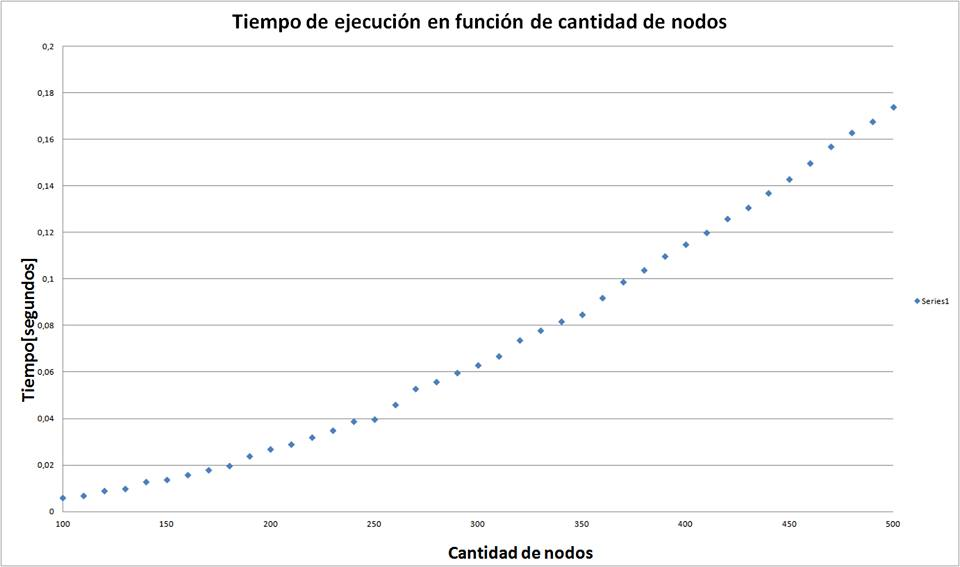
\includegraphics[scale=0.5]{imagenes/graph3.jpg}
\caption{Gráfico de tiempo de ejecución en función de la cantidad de nodos de la instancia}
\end{figure}

Dado que se nos solicitó que la complejidad temporal fuera estrictamente menor que O($n^3$), dividimos los tiempos obtenidos por la cantidad de nodos al cubo en cada caso. Como podemos ver en el siguiente gráfico, al realizar la comparación obtenemos una función con comportamiento decreciente, lo que muestra experimentalmente que nos ajustamos a la cota establecida.

\begin{figure}[H]
\centering
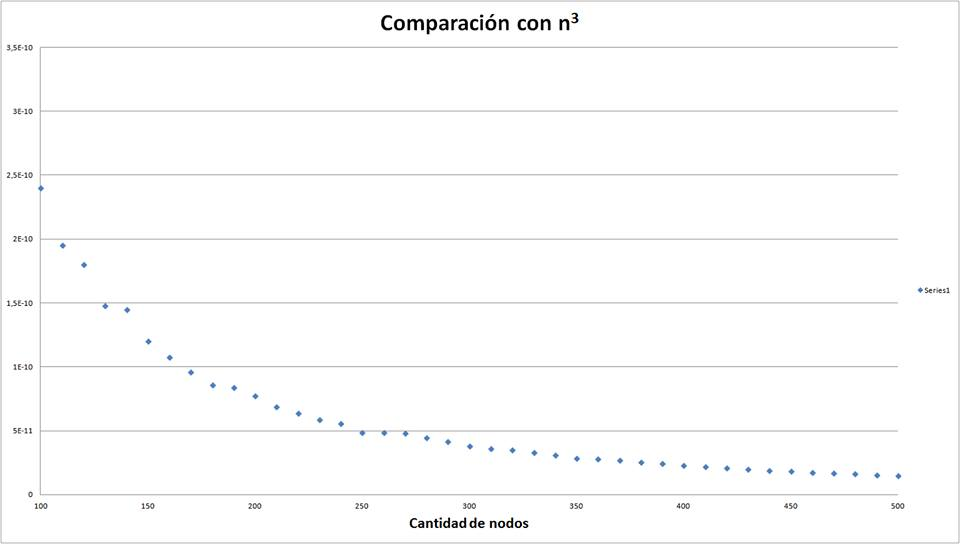
\includegraphics[scale=0.5]{imagenes/graph4.jpg}
\caption{Gráfico de comparación con $n^3$}
\end{figure}

Como propopusimos anteriormente, debido a que tenemos que ordenar todas las aristas del grafo, nuestro algoritmo está dominado por la complejidad del \textit{sort} de la STD y por lo tanto obtenemos una complejidad de O($n^2log(n^2)$. Para verificar esta afirmación (al menos en un conjunto de prueba), comparamos ahora los tiempos de ejecución con $nlog(n^2)$ esperando obtener una función lineal. Efectivamente fue lo que obtuvimos:

\begin{figure}[H]
\centering
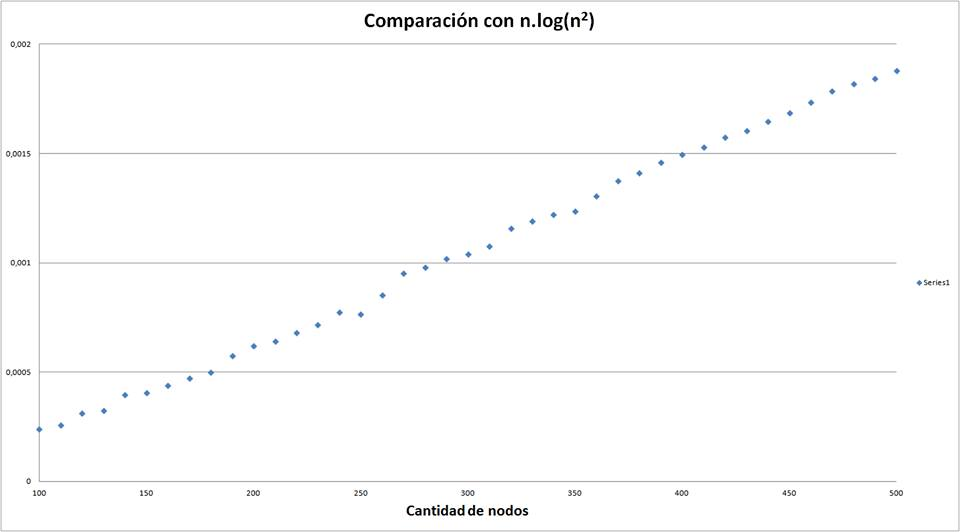
\includegraphics[scale=0.5]{imagenes/graph1.jpg}
\caption{Gráfico de comparación con $nlog(n^2)$}
\end{figure}

Consideramos que las desviaciones que se perciben corresponden a alteraciones en la ejecución debido al uso de CPU en ese momento y no dependen de la instancia. Una forma posible de reducir este tipo de errores consiste en, por ejemplo, repetir la medición en distintos momentos y tomar un promedio.

Debido a que el comportamiento de la función \textit{sort} ya fue analizado en un trabajo previo, para esta experimentación nos enfocamos en los algoritmos implementados por nosotros. Tanto el algoritmo que arma el AGM (prim) como el que busca el ciclo sólo toman en cuenta la cantidad de nodos del grafo y, por lo tanto, analizar diferentes familias de casos no aportaría aspectos interesantes de los mismos. Sin embargo, en los casos en los que no hay solución sí pudimos encontrar instancias en los que el chequeo resulta inmediato y casos en los que no para grafos con la misma cantidad de nodos. 

Recordemos que para el problema planteado, si la red de la entrada no es conexa o es un camino simple, el problema no tiene solución. Mientras que la detección de caminos simples o conectitud para grafos de pocas aristas resulta muy rápida, a medida que aumentan las aristas, esta detección se vuelve cada vez más lenta. Así, para casos de entre 100 y 500 nodos, detectar un camino simple o  falta de conectitud con pocas aristas (menos aristas que nodos) consume menos de $0.001$ segundos en todos los casos. Sin embargo, si tomamos el caso extremo de no conectitud ($K_{n-1}$),
en donde queda un nodo aislado, la situacion es diferente, como podremos apreciar en el siguiente grafico:

\begin{figure}[H]
\centering
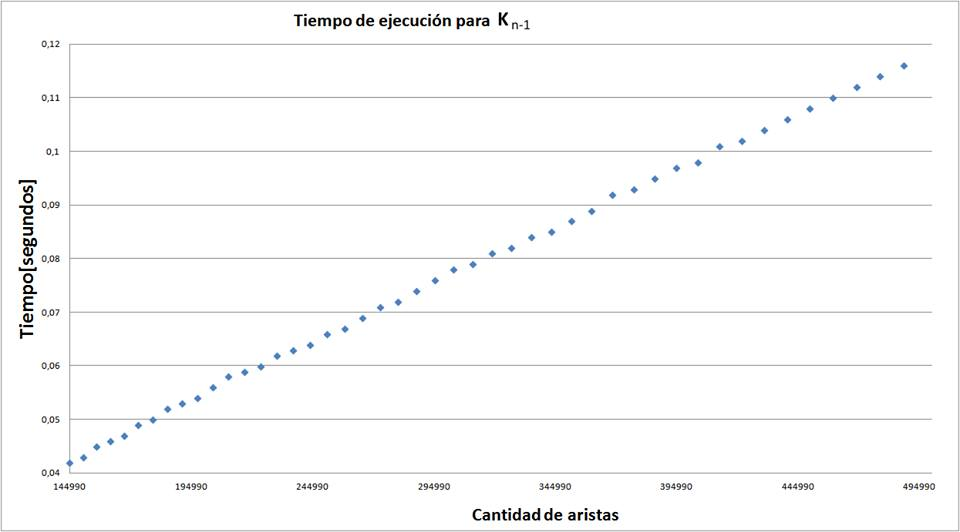
\includegraphics[scale=0.5]{imagenes/graph2.jpg}
\caption{Gráfico de tiempo de ejecución para instancias grandes sin solución}
\end{figure}


Podemos ver entonces que el algoritmo empleado para detectar conectitud se ve afectado por la cantidad de aristas en el grafo. En particular, su tiempo es lineal respecto a la cantidad de aristas.


\subsection{Adicionales}

En una nueva versión del problema se nos solicita una solución para el caso en el que un enlace cambie su costo. Se nos pide que aprovechemos la solución obtenida y se nos consulta sobre el impacto de esta modificación en la complejidad.

Para este caso, sea $f$ la arista que se modifica. Si la agregamos al AGM $T$ que nos devuelve Prim, generariamos un ciclo. Si de ese ciclo eliminamos la arista de menor peso, tendriamos el nuevo AGM correspondiente a la red con ese enlace modificado. Luego podríamos resolver de la misma manera que antes, con la salvedad que, en lugar de volver a ordenar todas las aristas de G, podríamos insertar $f$ en el lugar correspondiente en el vector de aristas. 

Esta modificación agrega el costo de construir un ciclo y el de insertar en forma ordenada. Para construir el ciclo vimos que necesitamos usar BFS que en nuestro caso tarda $O(n^2)$. Para agregar ordenado en un vector tendríamos que copiar el mismo, por lo tanto, tenemos tiempo lineal en el tamaño del vector, osea $O(n^2)$ dado que se trata del vector de aristas (que son $n^2$ en el peor caso). 

Dicho esto, la complejidad teórica del algoritmo no se modifica ya que todas las operaciones siguen costando menos que $O(n^2log(n^2))$.

%% =====================================================================

\end{document}
